%%
% BIThesis 本科毕业设计论文模板 —— 使用 XeLaTeX 编译 The BIThesis Template for Undergraduate Thesis
% This file has no copyright assigned and is placed in the Public Domain.
%%

% 第一章节
\chapter{实验设计与结果分析}

\section{实验设计}

\subsection{开发环境配置}

\textcolor{black}{实验使用如下开发环境:}

\textcolor{black}{(1)实体机操作系统及版本号:Windows10 22H2}

\textcolor{black}{(2)虚拟机软件,虚拟机操作系统:VMWare Workstation 16.1.2 build-17966106,Windows7 旗舰版
}

\textcolor{black}{(3)集成开发环境:PyCharm 2024.3.5 (Professional Edition) }

\textcolor{black}{(4)Python虚拟环境:Anaconda 24.11.3 AnacondaNavigator2.6.5 }

\textcolor{black}{(5)反病毒软件:主机安装Clam AV,建议手动更新病毒库到最新版本。虚拟机中安装火绒杀毒和360杀毒以备后续使用,本实验中不建议在主机上安装多个反病毒软件,因为可能会导致主机出现蓝屏崩溃问题,因此,其它用于后续使用的反病毒软件建议安装在虚拟机中。}

\textcolor{black}{(6)项目依赖位于项目根目录下的requirements.txt文件中,可以使用anaconda直接导入requirements.txt文件来创建Python虚拟环境。}

\textcolor{black}{(7)实体机存储:内存空间 32GB,磁盘空间 512GB}

\subsection{原始样本获取}

\textcolor{black}{首先,在开始实验前,需要提前收集足够量的恶意样本以供本实验使用,针对此问题的解决方案是从国外VirusShare的开放恶意样本库,以及部分国内安全软件论坛,例如火绒杀毒,360杀毒等官方论坛,收集并且下载恶意样本。本实验中大约使用2000个恶意样本,并将它们分为五组以备后续使用。如果是在Virus Share上收集,需要注意文件的类型,需要是PE可执行文件。}

\textcolor{black}{用于对抗性操作的无害程序,主要用于增加伪造的签名,无害段等对抗性操作,这些无害程序的获取方式,可以从国内一些软件公司的软件安装包获取,使用sigthief将签名剥落,关于sigthief的具体使用可以参考https://github.com/secretsquirrel/SigThief 的readme的相关说明,这些从良性程序剥落下的签名可以从一些官方途径下载的软件安装包可执行文件中剥落下来。用于增加无害段需要收集一些良性DLL文件,可以从Windows操作系统根目录下的一些DLL文件中获取。}

\subsection{配置VMWare虚拟机}

\textcolor{black}{需要创建实验用Windows7虚拟机并安装VMware Tools,并调整360杀毒相关设置关闭不需要的反病毒引擎,取消勾选系统修复引擎、behavioral脚本引擎,鲲鹏引擎,避免对实验结果造成干扰。同时,需要注意潜在的样本污染问题,对于360杀毒,需要关闭自动上传发现的可疑文件,取消勾选自动上传发现的可疑文件,否则可能导致有些样本被360杀毒上传到云查杀服务器数据库中,导致后续结果查杀率偏高的问题。}

\textcolor{black}{需要注意的是,安装360杀毒后需要重启虚拟机以保证360杀毒相应查杀服务开启,否则会导致实验结果出现偏差。}

\textcolor{black}{本实验不会测试360杀毒的鲲鹏引擎,是因为大多数反病毒软件,倾向于防御现有的威胁和威胁变种,而不是没有广泛传播的对抗性样本,鲲鹏引擎也如此,它多被360杀毒用于对抗目前广泛流行的恶意样本(例如银狐和某些流行的勒索病毒),而非对抗性样本或是离目前时间较久远的样本,而且鲲鹏引擎几乎没有机器学习的自学习能力,但QVM引擎具有机器学习能力,很明显,QVM引擎更适合用于本次实验的结果检验。这是因为有时需要反病毒软件对未知程序的判断更加精准以及判断速度更快,也就是尽量降低误报的可能性以及判断时间。为了减少误报率,很多反病毒软件厂商可能会使用白名单数字签名放行,或是使用文件哈希白名单来进行放行。因为例如Intel、AMD的硬件驱动程序,它们会加载驱动,如果这些硬件外设驱动程序因为释放了一些驱动文件被反病毒软件误报没有放行,将会导致某些外设驱动不能正常安装,对用户来说后果无疑是灾难性的,极有可能导致操作系统或是计算机崩溃。但这些硬件驱动程序跟某些病毒的行为很相似,某些病毒也会使用驱动来提升自己的操作权限,使自己具有更强的破坏力以及更好地针对和破坏反病毒软件,因此,对于这些驱动程序以及一些驱动安装工具,大多数反病毒软件会选择单独白名单规避此类问题。同时,360杀毒的behavioral脚本查杀引擎和系统修复引擎也需要关闭防止造成检出率偏高导致误差。}

\subsection{结果评估标准}

\textcolor{black}{首先,定义查杀率如下:}

\textcolor{black}{查杀率计算公式如式4-1:}
\begin{equation}
P_{detect\_rate}=m_{detect\_sample\_amount}/m_{total\_sample\_amount}
\end{equation}

\textcolor{black}{对于某个恶意软件集合$sample\ s_{\omega}$,某反病毒软件的查杀率被定义为经该反病毒软件扫描该恶意软件样本集合的检出恶意软件数量除以恶意软件集合中总恶意软件数量。}

\textcolor{black}{为了更好计算样本集的规避反病毒软件的查杀效果,使用该公式要求原始样本和生成的对抗性样本前后都使用同一款反病毒软件进行扫描,则查杀下降率定义如式(4-2)所示:}
\begin{equation}
\delta_{decline\_rate}=(P_{detect\_rate\_before}-P_{detect\_rate\_after})/P_{detect\_rate\_before}
\end{equation}

\textcolor{black}{语言描述为:查杀下降率=(原始样本检出率-处理后样本检出率)/原始样本检出率。}

\textcolor{black}{Virus Total检出率的定义为式(4-3)所示: }
\begin{equation}
P_{detect\_rate}=m_{detect\_engine\_amount}/m_{total\_engine\_amount}
\end{equation}

\textcolor{black}{对于某个恶意软件样本,VirusTotal检出率定义为检出引擎总数/Virus Total扫描引擎总数。}

\textcolor{black}{Virus Total检出率的下降率定义如式(4-4)所示:}
\begin{equation}
    \delta_{decline\_rate}=(P_{detect\_rate\_before}-P_{detect\_rate\_after})/P_{detect\_rate\_before}
\end{equation}

\textcolor{black}{对于某个恶意软件样本,VirusTotal检出率的下降率定义为(原始样本VirusTotal检出率-处理后样本VirusTotal检出率)/原始样本VirusTotal检出率。}

\section{实验结果}

\textcolor{black}{在本次实验中,一共使用了五组样本集,合计大约2000个样本来进行测试,测试结果如下所示。对于处理前的原始样本集和处理后的样本集,分别使用前文中配置好的恶意程序扫描模块和手动上传至虚拟机使用火绒杀毒和360杀毒扫描,并且随机选取一些原始样本和对应的处理后样本上传VirusTotal进行分析。值得注意的是,获取实验结果数据时,在虚拟机中使用360杀毒和火绒对样本扫描之前,需要关闭虚拟机中的反病毒软件,再在主机上使用XFTP等软件或VMwareTools拖拽向虚拟机中发送样本集,防止样本集发送过程中受到反病毒软件的干扰和潜在的数据污染问题,例如360杀毒会默认禁止存在风险的远程主机向本主机的FTP协议,在本次实验中对于虚拟机不需要这个防御功能。且在主机和虚拟机的FTP协议或VMWareTools拖拽完成文件传输后,虚拟机接收到文件后,360杀毒会自动扫描文件,这是不应该被允许的。因为会导致后续检出率偏高以及360杀毒等反病毒软件会直接隔离虚拟机接收到的样本集中的一些样本,对后续统计查杀数量带来了不便。}

\subsection{实验结果的数据图示}

\textcolor{black}{五组样本集处理前后的扫描结果图\ref{fig:sample1}、图\ref{fig:sample2}、图\ref{fig:sample3}、图\ref{fig:sample4}、图\ref{fig:sample5}、图\ref{fig:Virus_Total}、图\ref{fig:compare_with_different_model}所示,对其具体分析将在后续章节中进行。}

\begin{figure}[htbp]
  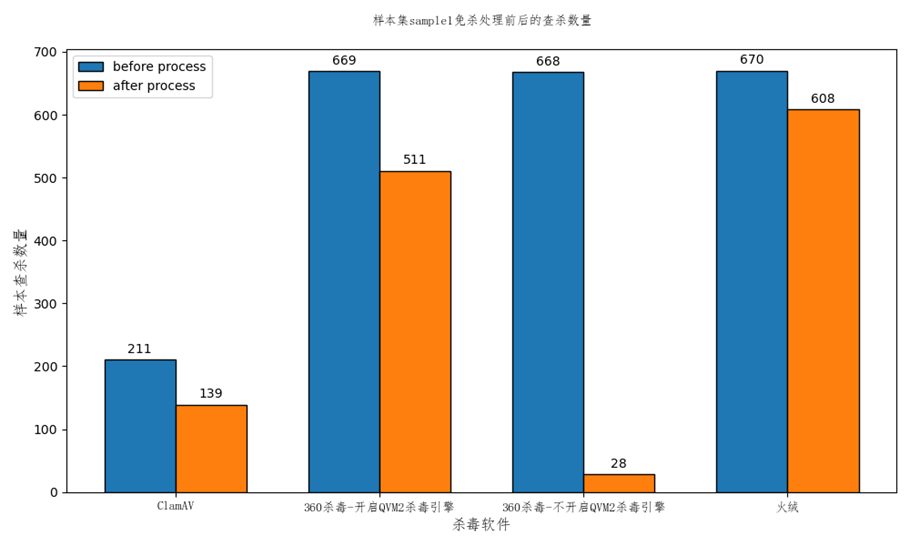
\includegraphics[scale=0.60]{images/sample1.png}
  \caption{sample1}\label{fig:sample1}
\end{figure}
\begin{figure}[htbp]
  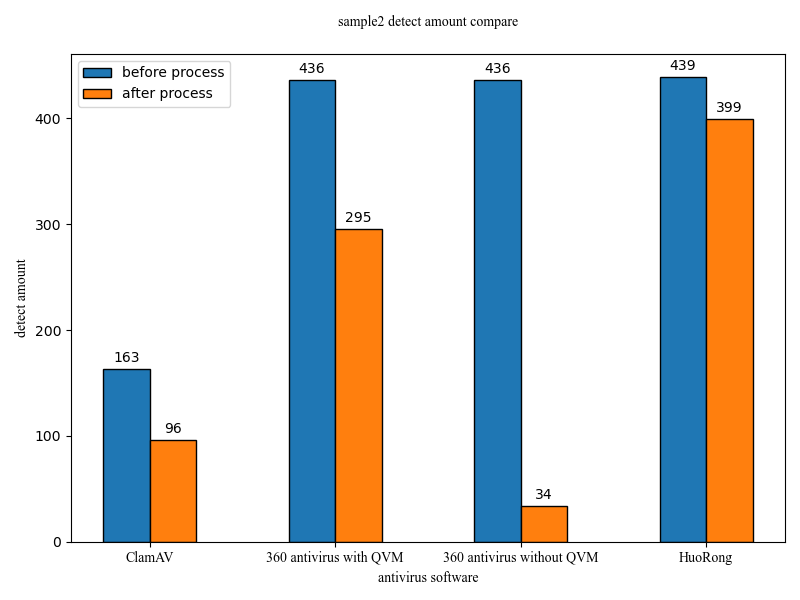
\includegraphics[scale=0.60]{images/sample2.png}
  \caption{sample2}\label{fig:sample2}
\end{figure}
\begin{figure}[htbp]
  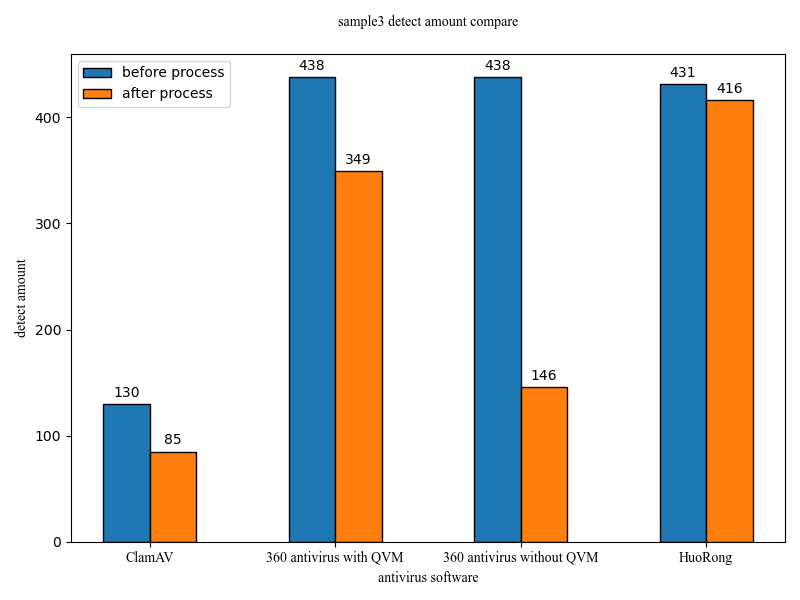
\includegraphics[scale=0.60]{images/sample3.png}
  \caption{sample3}\label{fig:sample3}
\end{figure}
\begin{figure}[htbp]
  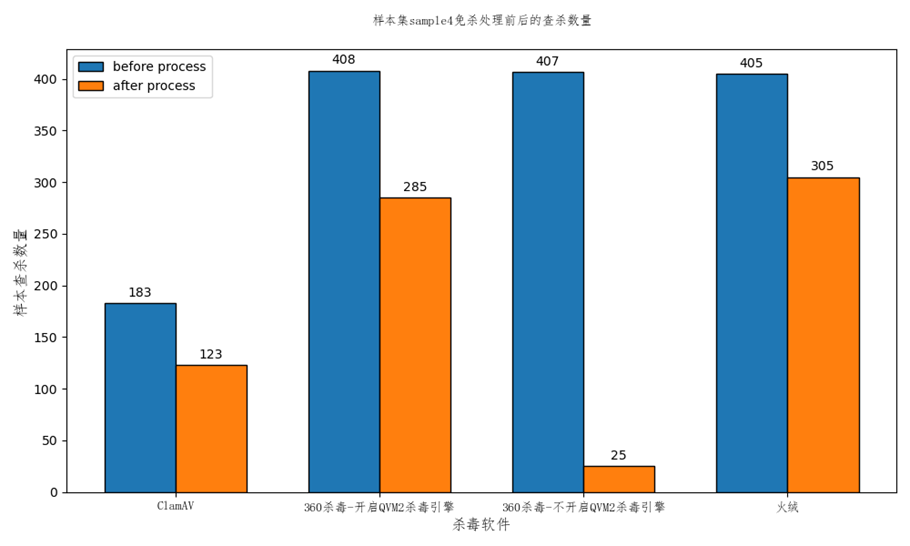
\includegraphics[scale=0.60]{images/sample4.png}
  \caption{sample4}\label{fig:sample4}
\end{figure}
\begin{figure}[htbp]
  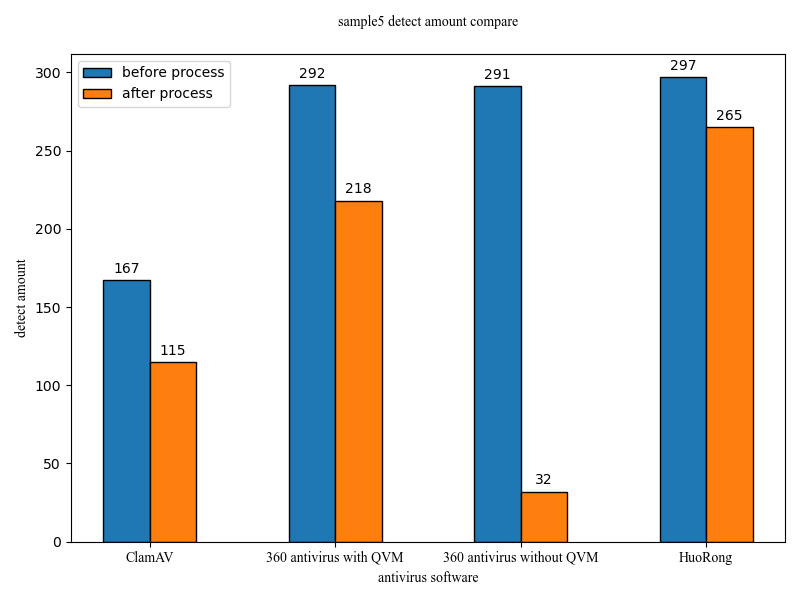
\includegraphics[scale=0.60]{images/sample5.png}
  \caption{sample5}\label{fig:sample5}
\end{figure}
\begin{figure}[htbp]
  \centering
  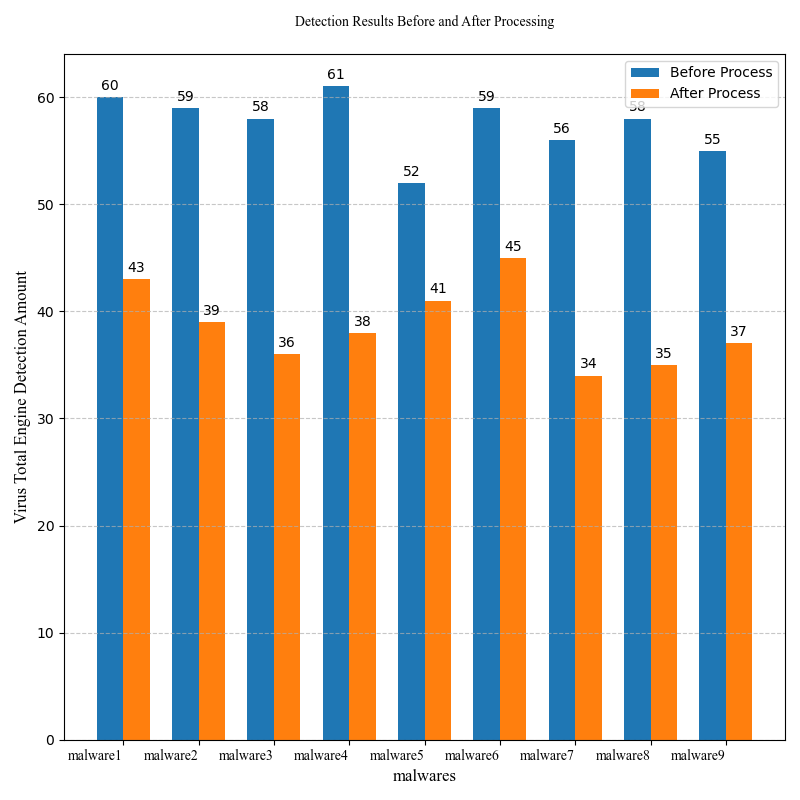
\includegraphics[scale=0.6]{images/Virus_Total.png}
  \caption{Virus Total}\label{fig:Virus_Total}
\end{figure}
\begin{figure}[htbp]
  \centering
  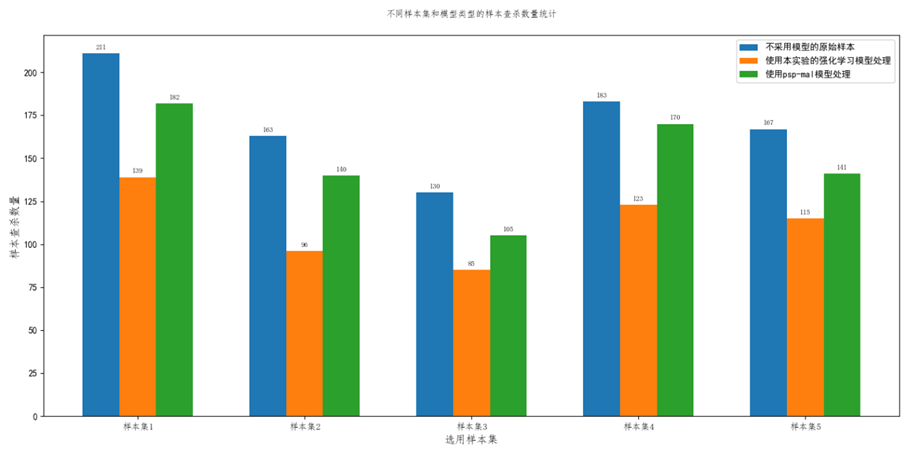
\includegraphics[scale=0.6]{images/compare_with_different_model.png}
  \caption{detect comparison of different models}\label{fig:compare_with_different_model}
\end{figure}
\subsection{检出率及其变化的计算}

\textcolor{black}{首先,对于某组样本中的随机抽样的部分程序,本实验中使用了Virus Total来进行上传扫描。}

\textcolor{black}{经过对图\ref{fig:sample1},图\ref{fig:sample2},图\ref{fig:sample3},图\ref{fig:sample4},图\ref{fig:sample5}中的数据进行计算,可以发现:}

\textcolor{black}{(1)对于样本集sample1:}

\textcolor{black}{Clam AV对本实验强化学习模型处理前后的样本检出率从31.3\%下降到了20.7\%;开启QVM杀毒引擎的360杀毒对本实验强化学习模型处理前后的样本检出率从99.3\%下降到了75.8\%;只开启360云查杀引擎,不开启QVM杀毒引擎的360杀毒对强化学习模型处理前后的样本检出率从99.1\%下降到了4.2\%;火绒杀毒对本实验强化学习模型处理前后的样本检出率从99.4\%下降到了90.2\%。}

\textcolor{black}{(2)对于样本集sample2:}

\textcolor{black}{Clam AV对本实验强化学习模型处理前后的样本检出率从37.4\%下降到了22.0\%;开启QVM杀毒引擎的360杀毒对本实验强化学习模型处理前后的样本检出率从100\%下降到了67.7\%;只开启360云查杀引擎,不开启QVM杀毒引擎的360杀毒对本实验强化学习模型处理前后的样本检出率从100\%下降到了7.8\%;火绒杀毒对本实验强化学习模型处理前后的样本检出率从100\%下降到了91.5\%。}

\textcolor{black}{(3)对于样本集sample3:}

\textcolor{black}{Clam AV对本实验强化学习模型处理前后的样本检出率从29.5\%下降到了19.3\%;开启QVM杀毒引擎的360杀毒对本实验强化学习模型处理前后的样本检出率从99.5\%下降到了79.3\%;只开启360云查杀引擎,不开启QVM杀毒引擎的360杀毒对本实验强化学习模型处理前后的样本检出率从99.5\%下降到了33.2\%;火绒杀毒对本实验强化学习模型处理前后的样本检出率从98.0\%下降到了94.5\%。}

\textcolor{black}{(4)对于样本集sample4:}

\textcolor{black}{Clam AV对本实验强化学习模型处理前后的样本检出率从44.9\%下降到了30.1\%;开启QVM杀毒引擎的360杀毒对本实验强化学习模型处理前后的样本检出率从100\%下降到了69.9\%;只开启360云查杀引擎,不开启QVM杀毒引擎的360杀毒对本实验强化学习模型处理前后的样本检出率从99.8\%下降到了6.1\%;火绒杀毒对本实验强化学习模型处理前后的样本检出率从99.3\%下降到了74.8\%。}

\textcolor{black}{(5)对于样本集sample5:}

\textcolor{black}{Clam AV对本实验强化学习模型处理前后的样本检出率从57.2\%下降到了39.7\%;开启QVM杀毒引擎的360杀毒对本实验强化学习模型处理前后的样本检出率从100\%下降到了74.7\%;只开启360云查杀引擎,不开启QVM杀毒引擎的360杀毒对本实验强化学习模型处理前后的样本检出率从99.7\%下降到了11.0\%;火绒杀毒对本实验强化学习模型处理前后的样本检出率从100.0\%下降到了90.8\%。}

\textcolor{black}{根据查杀下降率的定义,对于五个样本集合的查杀下降率计算结果如下表\ref{chart1}中所示: }

\begin{table}[htbp]
  \centering
  \caption{查杀下降率结果}\label{chart1}
  \begin{tabular}{*{6}{>{\centering\arraybackslash}p{2cm}}} \toprule
    反病毒软件类型/样本    & sample1    & sample2    & sample3   & sample4    & sample5   \\ \midrule
    ClamAV    & 34.1\%  & 41.1\% & 34.6\%  & 32.8\%  & 31.1\%\\ \midrule
    360杀毒开启云查杀引擎和QVM引擎   & 23.6\%  & 32.3\%  & 20.3\%  & 30.1\%    & 25.3\%\\ \midrule
    360杀毒开启云查杀引擎不开启QVM引擎 & 95.8\%  & 92.2\%  & 66.7\%  & 93.9\%    & 89.0\%\\  \midrule
    火绒 & 9.3\%  & 9.1\%  & 3.5\%  & 24.7\%    & 10.8\%\\ \bottomrule
    \end{tabular}
\end{table}

\textcolor{black}{计算平均值如表\ref{chart2}中所示:}

\begin{table}[htbp]
  \centering
  \caption{查杀下降率结果平均值}\label{chart2}
  \begin{tabular}{*{2}{>{\centering\arraybackslash}p{2cm}}} \toprule
    ClamAV    & 34.74\%\\ \midrule
    360杀毒开启云查杀引擎和QVM引擎   & 26.32\%\\ \midrule
    360杀毒开启云查杀引擎不开启QVM引擎 & 87.52\%\\  \midrule
    火绒 & 11.48\%\\ \bottomrule
    \end{tabular}
\end{table}

\textcolor{black}{从结果中看出,对抗性样本对于不同反病毒软件的有效性,对360云查杀引擎最有效,对火绒的有效性最差。}

\textcolor{black}{前文中图\ref{fig:Virus_Total}使用Virus Total扫描上传从某个样本集合内随机抽样的PE恶意程序,在云端总共使用了70余个反病毒软件进行分析。}

\textcolor{black}{处理前后检出率变化以及检出下降率变化如表\ref{chart3}所示:}

\begin{table}[htbp]
  \centering
  \caption{查杀下降率结果平均值}\label{chart3}
  \begin{tabular}{*{4}{>{\centering\arraybackslash}p{2cm}}} \toprule
    样本/检出率    & 处理前检出率  & 处理后检出率  & 检出下降率\\ \midrule
    malware1   & 83.3\%  & 59.7\%  & 28.3\%\\ \midrule
    malware2 & 80.8\%  & 54.2\%  & 33.0\%\\  \midrule
    malware3 & 79.5\%  & 50\%  & 37.1\%\\  \midrule
    malware4 & 83.6\%  & 53.5\%  & 36.0\%\\  \midrule
    malware5 & 71.2\%  & 56.9\%  & 20.0\%\\  \midrule
    malware6 & 81.9\%  & 61.6\%  & 24.8\%\\  \midrule
    malware7 & 77.8\%  & 47.2\%  & 39.3\%\\  \midrule
    malware8 & 80.6\%  & 48.6\%  & 39.7\%\\  \midrule    
    malware9 & 75.3\%  & 51.4\%  & 31.8\%\\ \bottomrule
    \end{tabular}
\end{table}

\textcolor{black}{且经过统计,当最大允许处理次数设置为16时,对于样本集sample1的处理总共花费12463.1秒,对于单个样本的平均处理时间为18.49秒。}

\textcolor{black}{样本集1样本大小变化率的散点图如图\ref{fig:scatter_of_sample1}所示,大小变化率的定义为对于某个确定的样本,其处理后的大小除以处理前的大小,可以发现,有少数处理后的样本大小变的较大,甚至可能会达到1000倍以上,这可能是因为添加节所选取的良性DLL文件中的.text节过于庞大导致的。}

\begin{figure}
  \centering
  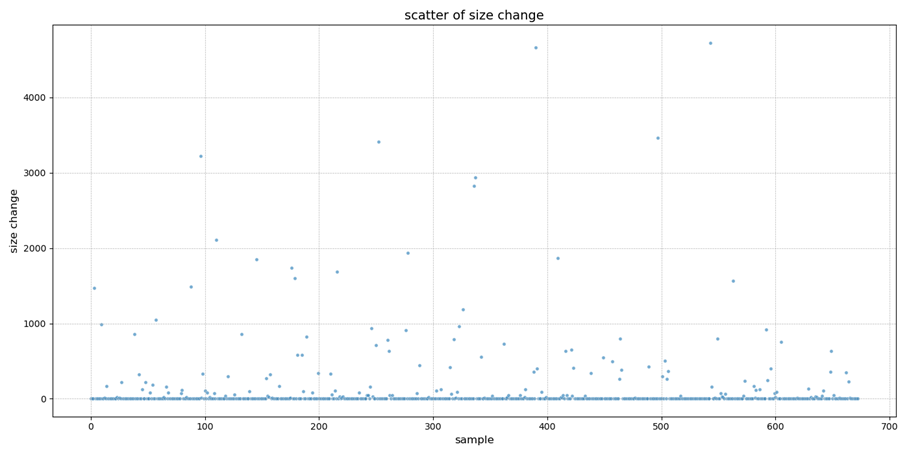
\includegraphics[]{images/scatter_of_sample1.png}
  \caption{scatter of sample1}\label{fig:scatter_of_sample1}
\end{figure}

\subsection{不同反病毒软件对于检出率变化的影响}

\textcolor{black}{处理后的样本对于火绒杀毒来说,表\ref{chart1}中数据计算出的逃逸概率低的原因是火绒有一定的反扰动能力,处理后的样本很多都会判断为:病毒类型-代码混淆器,火绒认为处理后的样本的某些特征是为了规避静态检测过程。说明有一部分反病毒软件的静态特征分析能力,能识别出对抗样本中的扰动。这也是为什么采用Sarsa算法不宜设置过大的state数值的原因,一方面是处理前后的PE程序反复读写,当程序大小因为新增节,新增无意义尾部内容,用无意义字节填充空洞等操作多次使用后变的过于庞大(在某次样本处理时,发现一个PE程序处理前后,变为原大小大约6.6倍,从2.67 MB变成了17.6MB),如果不限制state值,程序中途会变得很大,不但导致后续的对抗性样本生成的干扰操作极其缓慢,因为要先读取原文件,然后再加以修改,最后写入磁盘中,Python对于文件的操作是很缓慢的。而且会导致根据查杀结果获取result的速度相当慢,因为Clam AV反病毒软件扫描一个样本的时间也和样本大小正相关,当样本很大的时候,判断查杀结果会相当的慢。另一方面,就是当无意义尾部内容过多,会被反病毒软件认为是疑似恶意程序刻意扰动,从而直接判定此程序为为了绕过反病毒软件检查的恶意程序。而从火绒杀毒对于样本的描述也可以看到这一点,火绒杀毒认为经过处理后的某些恶意程序是代码混淆器。同时,火绒查杀结果总数量会略高于样本数量,原因目前未知。}

\textcolor{black}{同样对于Clam AV,可知它的部分检测也能识别对抗样本中的扰动性操作,尽管经过处理后的恶意程序中有大量良性内容,但Clam AV仍然会查杀这些恶意程序。}

\textcolor{black}{由此可见,部分反病毒软件对于静态规避操作的对抗性扰动有一定的抵抗,会造成处理前后检出率变化较小。}

\textcolor{black}{但QVM引擎对于对抗性扰动能力偏弱,这是因为QVM引擎作为一个自学习的人工智能引擎,这个病毒检测引擎是基于机器学习的模型,通过检测文件的某些特征,来判断该文件是否是恶意程序,如果某程序被QVM引擎检测出是恶意程序,那么360杀毒在查杀结果中会报HEUR/QVM.xx.Malware.Gen字样。这里使用QVM引擎作为检测标准是为了研究论文中的强化学习对抗性样本生成模型产生的处理后静态检测规避对抗性样本在基于不同模型的反病毒软件之间的逃逸可迁移性,以及验证机器学习的病毒检测引擎对于静态检测规避对抗性样本的抗干扰能力。但遗憾的是,QVM引擎对于静态检测规避对抗性样本的抗干扰能力比较差,有时甚至仅仅增加了无意义的图标ICO资源,QVM引擎就认为样本是良性的。}

\subsection{与psp-mal模型的对比}

\textcolor{black}{如图\ref{fig:compare_with_different_model},可以发现本实验强化学习模型处理后的样本集,相比psp-mal模型,能更好规避ClamAV反病毒软件的查杀,原因可能是新增的伪造签名操作,增加无关资源操作,和UPX加壳等操作导致的。检出率的变化对比如表\ref{chart4}所示,值得注意的,不同于本实验中使用了Sarsa强化学习算法,psp-mal模型使用的方法是沙普利先验,检验是否逃逸成功使用的是SOREL-20M和EMBER反病毒模型,遗憾的是,通过对图\ref{fig:compare_with_different_model}的分析,可以知道psp-mal模型的可迁移性较差,尽管psp-mal模型生成的对抗性样本能逃脱EMBER反病毒模型,但是对于ClamAV的查杀来说,规避性能较差,甚至检出率变化不足20\%。由此可见,本实验设计的创新点有利于对抗性样本的迁移,能达到对不同反病毒软件的静态检测逃逸效果。}

\begin{table}[htbp]
  \centering
  \caption{检出率变化对比}\label{chart4}
  \begin{tabular}{*{3}{>{\centering\arraybackslash}p{2cm}}} \toprule
    样本集/检出率变化    & 本实验中强化学习模型  & psp-mal\\ \midrule
    sample1   & 34.1\%  & 13.7\%\\ \midrule
    sample2 & 41.1\%  & 14.1\%\\  \midrule
    sample3 & 34.6\%  & 19.2\%\\  \midrule
    sample4 & 32.8\%  & 7.1\%\\  \midrule
    sample5 & 31.1\%  & 15.6\%\\ \bottomrule
    \end{tabular}
\end{table}

\subsection{静态对抗性样本对云查杀的影响}

\textcolor{black}{相对于传统的对抗性样本需要恶意攻击者手动修改自身的恶意程序二进制代码,繁琐低效,而且可能因为修改失误导致恶意程序受损,产生对抗型样本的数量少,基于人工手动修改的对抗性样本难以对抗反病毒软件的云查杀,人工手动修改的变种终究只有少量。而本实验基于强化学习的Sarsa模型自动生成对抗型样本,对于单个恶意程序,能产生的对抗性样本数量较大,当变种数量足够多时,在有限的时间内,反病毒软件的云查杀系统未必能全部识别出。大量的对抗型样本对云查杀的压力也是较大的。}

\textcolor{black}{为了研究云查杀对于检出率的影响,需要在VMware创建的Windows7虚拟机中使用360杀毒进行测试静态检测规避对抗性样本的查杀情况且在360杀毒的设置中打开了自动上传发现的可疑文件。在结果中发现尽管部分处理后的样本逃逸了360杀毒的自定义查杀的检出,但是360杀毒仍然将这些逃逸样本归类为可疑文件。虽然这些逃逸样本不会报为高危风险项,但是360杀毒仍然会将这些样本上传到360云安全中心来进行检验,在可疑样本被360杀毒上传之后的一段时间,再次启动自定义查杀扫描剩余的逃逸样本,有部分样本被360杀毒检出判定为高危风险项。说明对于开启未知程序上报的云查杀(360云安全中心具有有动态行为检测的,并不完全只有静态检测)的安全软件来说,对抗性样本攻击虽然有一定危害,但大多数仍然最终会被检出是恶意程序。同时,360杀毒也具有动态检测功能,例如Behavioral脚本引擎、主动防御模块这些基于动态行为分析的检测,如果用户执行了恶意程序,360杀毒会拦截并且隔离恶意程序。当反病毒软件具有动态检测功能,则静态对抗性样本攻击的效果是有限的,但仍然不可以忽视。究其原因,是因为某些具有反虚拟化策略、反沙箱、识别监控进程的功能的病毒已经被指出可以逃逸动态检测。\cite{ref33}\cite{ref34}\cite{ref35}\cite{ref36}}

\textcolor{black}{云查杀技术对这些病毒来说未必有效,因为在被上传到云端沙箱(例如Cuckoo Sandbox)中之后,恶意软件不会表现出预期的恶意行为,从而阻碍了恶意软件行为分类和恶意行为的自动识别检测。过度依赖云查杀仍然可能会存在潜在的威胁,同时,云查杀需要联网访问云端恶意软件样本数据库的问题也是一大安全隐患,对抗性恶意程序可能在自己被运行时,因为反病毒软件因为对抗性恶意程序自身的扰动导致判断该恶意程序是未知安全性,判断后需要上传到云端服务器,来利用云查杀技术进行分析,而这时的恶意程序自身可能会通过修改网络设置导致计算机无法连接到互联网,或利用Windows防火墙规则,本地Hosts文件篡改反病毒软件请求服务器地址到本地环回地址127.0.0.1等方式,使反病毒软件无法连接到互联网,从而阻止了反病毒软件从云端服务器获取云端沙箱检测等传回来的信息,这就导致反病毒软件对于对抗性恶意程序无法进行精确地判断是否具有恶意性。更糟的情况是当云查杀技术面对未来可能出现的感染型病毒变种对抗性样本和蠕虫对抗性样本。}

\textcolor{black}{传统的感染型病毒,例如文件型病毒,只感染固定的目标文件\cite{ref37},例如PE可执行文件(.exe),动态链接库文件(.dll),html文件(.html/.htm),以及目前发现的一些宏病毒,只感染office文件,例如后缀为docx、xlsx、pptx、xls、doc、ppt的文件等。}

\textcolor{black}{其中的一部分传统感染型病毒,通过将自身的代码附加在正常程序后来感染正常程序。当程序被运行时,其中的病毒代码也随之运行。然而,传统的感染型病毒很容易被反病毒软件查杀,因为反病毒软件只需要进行全盘扫描,扫描文件系统中的所有文件来寻找已被病毒感染的文件,通过静态分析,检查其尾部内容是否有病毒库中黑名单的恶意代码字段,即可判断这个文件是否已经被感染型病毒所感染。而且反病毒软件对被感染的文件可以通过匹配相应二进制字符串,如通过正则表达式匹配,从而直接去除截断掉尾部的病毒代码进行文件修复。因为病毒代码和正常程序代码是物理分离的,所以反病毒软件的操作可以将受感染型病毒感染的文件恢复到原始文件状态,即对被感染的文件实行修复而不是直接删除或者隔离,可以使被感染的文件保留其原始正常文件的功能。}

\textcolor{black}{然而,通过本实验,可以说明,将来很可能存在某种感染型病毒变种对抗性样本。不同于传统的感染型病毒,它的危害相对较大,本身具有感染新文件后,自身也会突变不断制造新变种的新型攻击方式。这种病毒除了自身的恶意代码,也携带了对抗性扰动操作的相关模块,例如产生一个内部包含被pyinstaller打包的附带Python编译的PE可执行文件,用于产生静态检测对抗性扰动来针对基于机器学习和深度学习的反病毒软件以实现逃逸静态检测的查杀。该变种对抗性样本的部分行为可用程序流程图表述,如图4-9所示,图4-9为该变种对抗性样本的感染流程以及使被感染的文件规避静态检测流程,在病毒因为用户运行导致入侵未被病毒感染的系统后,该病毒会在磁盘中通过遍历文件系统的目录来寻找新的可被该病毒感染的目标文件,将自身代码附加在被感染程序后,并判断产生对抗性扰动操作的程序对应的$Environment\_Variable\_\alpha$环境变量是否存在,若存在则调用产生对抗性扰动的可执行程序对被新感染的程序进行处理,否则释放可产生对抗性扰动的可执行程序,随后将其移动到安装有操作系统的磁盘的某个位置(可以为系统根目录)下,随后设置文件为隐藏属性,添加该可执行程序到系统的环境变量中,最后调用产生对抗性扰动的可执行程序对被新感染的程序进行静态免杀处理,其伪代码描述如代码\ref{lst:cppfile1}所示。}

\begin{figure}
  \centering
  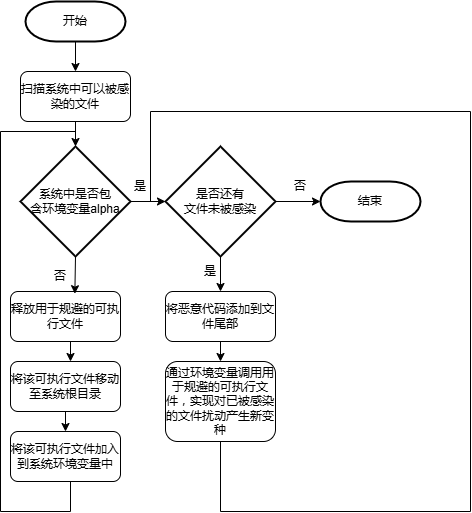
\includegraphics[]{images/attack.png}
  \caption{攻击过程}\label{fig:attack}
\end{figure}

\begin{lstlisting}[language=C++, caption={}, label={lst:cppfile1}]
/*
功能:感染型病毒变种入侵系统并感染可以感染的文件,在感染新文件时执行对抗性操作,被感染的新文件会受到静态规避操作的修改。
输入:无
输出:无
*/
start(); //病毒被运行  
scan_all_files_in_system_to_get_can_infected();   
function1:  
if System_Environment_Variables.contains(Environment_Variable_alpha){//检测到环境变量  
    for file in files_virus_can_infected{//感染过程  
        append_malicious_code(file);  
        run_evasion_module(Environment_Variable_alpha);  
    }  
}  
else{//释放对抗性操作文件及环境变量准备  
    release_executable_file_for_evasion();  
    move_evasion_module_file_to_system_root_folder();  
    add_environment_variable_to_system_environment_variables(Environment_Variable_alpha);  
    go to function1;  
}  

\end{lstlisting}

\textcolor{black}{这种感染型病毒变种每次新感染的程序的尾部病毒代码将互不相同,因为受到了对抗性扰动可执行程序的修改。基于静态分析的反病毒软件很难查杀这种变种对抗性样本,很容易面临能杀毒,但是查杀不完全的问题,每次杀毒如果不能检测出感染型病毒变种对抗性样本感染的全部文件,遗留下来的受感染文件一旦被用户无意间通过启动,例如通过某些Windows应用程序的开机自启动,用户打开浏览器访问网页但是浏览器主程序已被感染,仍然会导致其他文件被感染。更危险的是,被感染的文件难以像应对传统文件型病毒的修复措施,即精准去掉尾部的病毒代码来恢复原始文件。因为需要处理对抗性扰动新增的节和无效字节,甚至有可能是导入表被篡改,节表被修改的行为,一旦去除有偏差,则会导致受感染文件无法正常运行。因此反病毒软件极有可能无法通过黑名单中的病毒代码来计算线性偏移量,进而直接截断固定长度的尾部从而修复直接受感染文件,只能选择删除,这对用户来说是危害巨大的,因为很多的Windows软件包含了大量的动态链接库(.dll)文件和PE可执行文件(.exe),一旦某些动态链接库被反病毒软件删除后,这些软件极有可能无法正常运行。即使反病毒软件拥有云查杀功能,频繁上传大量变种样本不但消耗了用户带宽资源,而且变种样本因为每个被感染的实例的尾部特征值唯一,难以在第一次扫描中就被反病毒软件检测出是恶意程序,只会被定性为不流行的可疑文件,这导致对感染型病毒的响应延迟,很有可能会面对云查杀查杀病毒并不彻底的问题。这将是一种可能存在的高级持续性威胁(APT)。}

\textcolor{black}{幸运的是,即使面对这种将来可能存在的感染型病毒变种对抗性样本,因为它只有不断产生静态规避变种的功能,而没有不断产生动态规避变种的功能,反病毒软件的动态行为检测仍能在病毒程序未执行感染操作时触发,识别出恶意程序并警告用户。同时,PE文件的动态规避目前尚未出现规模化的攻击方法,尽管已有研究证明可通过代码分片来攻击动态行为检测\cite{ref38}\cite{ref39}\cite{ref40}。}

\textcolor{black}{同时,基于静态规避对抗性生成模型,未来也有可能会出现新的木马下载器变种,以及基于Web请求拦截器和对抗性生成模型挂马网站变种,这值得反病毒软件厂商警惕。许多网页框架,例如Java的SpringBoot CGI服务器,具有Interceptor接口用于拦截器操作,然而,这可以被黑客用于木马下载器来下载其他木马的静态规避变种,黑客可以使用SpringBoot的Interceptor接口确保每次访问挂马网站下载到的木马都是不同的。当木马下载器试图使用http的get请求访问黑客的挂马服务器来将木马下载到本地,这里假设为https://www.malicous.net/trojan\_file,在黑客对挂马服务器业务逻辑处理进行修改后,当服务器后端接收到对于trojan\_file子网页的请求,首先会被拦截器拦截,拦截器含有的业务逻辑会先将原始木马文件生成对抗性样本,然后,拦截器的业务逻辑会删除掉上一次生成的对抗性样本,使用新生成的对抗性样本对其覆盖,当对抗性操作结束后,拦截器放行请求,相对应的trojan\_file\_servlet对http请求进行处理,返回301状态码进行重定向操作,定向到挂马服务器上已经经过对抗性模型处理后的对抗性样本,在这里假设为https://www.malicous.net/trojan1\_modified.exe ,服务器返回静态对抗性木马trojan1\_modified.exe给木马下载器,随后,木马下载器将该文件保存到受害者的计算机上以备黑客后续入侵使用。尽管反病毒软件可能识别到了下载行为,但是下载的文件因为自身是静态分析对抗性样本,这会导致反病毒软件可能认为下载的文件是无恶意的文件。且木马下载器自身几乎不带有主动破坏计算机的恶意行为,只作为下载和启动其它木马的桥梁。此时,反病毒软件更多情况是认为木马下载器类似Motrix等的小型下载工具或者是正常程序的补丁更新,同时因为下载产生的数据流量不会过大,难以被判断为网络攻击。此时,相当于木马下载器完成了植入阶段的过程,在受害者的计算机上从黑客的挂马服务器上成功完成了下载木马程序。随后,将可能进入孵化期,上线期,攻击期\cite{ref41}。}

\textcolor{black}{幸运的是,反病毒软件可以根据网站安全可信度,并将某个IP或某个域名及其子域名下的所有内容划分为黑名单,禁止用户和应用程序访问。但不容忽视的是,域名和IP安全性鉴定仍然需要时间。虽然开始时木马下载器变种在植入阶段选择下载能逃逸反病毒软件静态分析的对抗型木马,避免自身因为下载恶意程序被反病毒软件直接判断为恶意软件,由此逃逸反病毒软件的检测,但反病毒软件随后仍然可以通过判断高风险http请求拦截木马下载器的危险请求,相比之下,基于静态分析对抗性的木马下载器变种危害性较小且反制难度小于感染型病毒变种对抗性样本。但不可忽视的是,黑客可以通过上述的变种挂马服务器,导致每个被木马感染的计算机的木马都是具有不同的Hash值且产生变种木马的原始木马样本被经过修改的操作组合不同,仅仅对单个原始木马程序经过前文中10种行为(Action)和16次step就可能存在$10^{10}$以上量级的变种,原始木马程序庞大的变种可以达到干扰甚至摧毁云查杀威胁情报的共享机制。}

\textcolor{black}{因此,在特定的条件下,如过度依赖本地静态检测忽视动态上传上报可疑文件、过度依赖云查杀的动态检测沙箱和云端病毒库遭遇网络中断、反病毒软件无条件直接信任某些公司签发的安全证书,很大可能会导致静态规避攻击绕过杀毒软件的防御,构成实际威胁。}

\subsection{静态对抗性样本对于动态检测技术的影响}

\textcolor{black}{尽管本实验的方案无法绕过动态检测,但静态规避研究仍具有重要价值,可以为用户执行潜在的恶意软件提供预判防御。动态规避属于另一个研究方向,目前shellcode的逃逸检测上已经出现了动态规避,通过异或加密shellcode后封装在C/Python代码的数组中,在执行时解密即可实现动态规避。然而动态检测相比静态检测,对某些恶意软件的检测效果并不佳,因为有些恶意软件会在运行时试图破坏反病毒软件,例如关闭相应的防御服务,加载驱动让自己常驻内存来对抗反病毒软件等操作,恶意软件针对反病毒软件的破坏行为需要反病毒软件的一些自我保护机制来应对,例如采用Intel-VT虚拟化技术(目前已被360安全卫士采用),HVCI内存防护技术。但遗憾的是,反病毒软件使用Intel-VT虚拟化技术会对用户运行VMware workstation、Virtual Box等虚拟机软件的流畅造成影响。同时,反病毒软件仍然需要考虑到许多服务器和个人电脑使用的老旧计算机硬件和操作系统官方宣布已经过时不再支持维护的操作系统,例如Windows2000、Windows XP操作系统,以及过时的Windows server操作系统Windows Server 2003,这些CPU和操作系统,由于发行时间较早,当时没有考虑到后续2005年之后Intel和AMD硬件厂商推出的硬件虚拟化技术,因此反病毒软件通过虚拟化技术的自我保护在这些过时系统上无法成功实现。尽管这些过时不再被微软支持维护的Windows操作系统的使用者在逐渐减少,然而,对于恶意攻击者而言,攻击这些微软不再提供安全更新和漏洞修复的系统相对于攻击Windows10和Windows11这种仍然被长期支持的操作系统而言更容易,也是部分恶意攻击者更加青睐的目标,因为目前几乎没有第三方机构愿意为这些过时的操作系统提供安全更新服务,这些过时的操作系统一旦被恶意攻击者发现漏洞并且针对漏洞编写木马程序,后果相比仍然被支持提供安全更新的操作系统是灾难性的。不能按照常理认为更多用户选用被支持提供安全更新的系统,因此恶意攻击者更倾向于攻击用户数更多的操作系统,事实上,仍有大量计算机由于数据迁移困难,硬件不合格,软件和驱动的支持问题,没有淘汰掉过时的操作系统,而这些操作系统有可能是木马和勒索病毒利用Windows通用漏洞攻击下发生的重灾区,在过去几年前的永恒之蓝漏洞就被勒索病毒WannaCry利用445端口针对几乎所有Windows操作系统的攻击。}

\textcolor{black}{因此,尽管动态检测对于静态规避类对抗型恶意程序样本对于计算机的攻击确实具有一定的阻止作用,且在阻止对抗恶意程序的运行时的恶意行为起到了重大作用,但仍然可能因为恶意程序对反病毒软件的破坏导致反病毒软件的动态检测丧失功能。且因为防御生态的割裂性,杀毒软件的自我保护功能在某些过时操作系统能否有效仍然是不确定的。}

\section{实验建议}

\subsection{对于相关研究人员}

\textcolor{black}{本研究使用对抗样本对采用机器学习技术的病毒查杀引擎进行黑盒测试,但需要注意,对某些特征的修改和删除,是否是修改容易被规避的脆弱特征、容易损坏原有恶意文件恶意行为的特征,例如机器码,本研究中尽管代码中保留了修改机器码的函数,但最终并未将其封装为操作函数,而是将其弃用,因为修改机器码在测试中并未通过,测试时使用了一个输出HelloWorld的C语言机器码为X86-64 PE可执行程序,在修改机器码后,导致程序无法执行、以及一些容易导致程序被直接查杀的特征,例如UPX加壳,在测试中,只采取UPX加壳,QVM引擎会直接判定该程序是恶意程序,甚至被UPX加壳的文件只是毫无危害的HelloWorld C语言程序。而采用UPX加壳以及多种方式混合,QVM引擎认为该程序是恶意程序的概率会大幅下降。同时,证明修改后的样本对计算机仍然有危害是至关重要的,但需要注意测试的安全问题,因为几乎没有一种杀毒软件能100\%的概率查杀静态处理后的样本,即使在测试中使用虚拟机,仍然可能会存在虚拟机逃逸问题,例如VMware WorkStation的漏洞CVE-2023-34048和CVE-2023-34056,测试前尽量对重要数据进行备份以及设置虚拟机还原点,防止运行恶意程序危害到实体机的意外发生。}

\subsection{对于反病毒软件厂商}

\textcolor{black}{本研究表明静态分析器容易被攻破,虽然目前没有出现前文中提及到的感染型病毒变种对抗性样本这种对静态分析针对性逃逸的流行性恶意软件,但规避静态分析的研究仍然具有价值,这也是为什么EMBER,MalConv等静态分析模型日益被关注的原因\cite{ref15},因为静态检测属于对恶意软件的第一道防线,保证能在用户执行恶意软件前就识别出恶意软件并且清除。}

\textcolor{black}{此外尽量不要过度依赖于本地病毒库的Hash值匹配病毒扫描策略,因为静态规避样本相比原样本Hash值不再相同,且达成静态检测规避的处理步骤不同,也会使不同的静态规避样本的Hash值不相同。同时,对某些异常PE可执行文件,例如尾部具有过长的字符串,可以考虑将它们判断为代码混淆器,疑似风险、不受欢迎文件提示给用户,并且上传到反病毒软件的云安全中心进行分析,而不是直接认为是无危害文件,尽管这样来说会有误报的可能,但是可以对抗一部分的规避静态分析的对抗性样本。例如ClamAV反病毒软件中允许开启的检测潜在不受欢迎程序(Potentially Unwanted Applications PUA)选项,虽然会误报一些用于计算机管理员监控计算机状态的网络嗅探、筛选工具和产生大量流量使用P2P网络的下载器程序,以及一些远程登录程序,JavaScript、ActiveX等类似语言编写的脚本、PC Hunter这种加载了驱动用于杀死进程的通用系统工具,但能检测出更多潜在恶意程序。此外,需要注意加强反病毒软件的自我保护功能和动态行为监测机制。同时,反病毒软件厂商也需要注意静态病毒库和动态病毒库的存放问题,本地可以尽量少存放静态病毒库,只存放一些近期流行的恶意程序样本,并且一段时间进行本地病毒库更新,这样可以为用户节省磁盘空间;而动态高风险动态行为检测库最好存放在本地,这样即使在网络环境不佳或者是离线状态,仍然能拦截病毒的运行,防止病毒危害计算机和造成用户损失。同时,云端病毒库可以对某些Hash值或者携带某些有效签名的程序的动态高风险行为设置白名单,例如一些签名注册工具。上述操作在网络正常的情况下,可以在经过本地高风险行为检测后,再进行云端查询判断程序是否是恶意程序,尽管会有离线模式下无法连接到云端病毒库导致误报某些非恶意软件的敏感操作的问题,但是可以很大程度上规避恶意程序运行造成的损失。在本实验中使用的Clam AV反病毒软件是基于本地离线病毒库,需要手动更新,大约有630MB大小。}

\section{本章小结}

\textcolor{black}{本章介绍了实验数据的具体来源以及实验环境配置,具体模块和具体功能的细节实现,采取了5组样本集进行实验并介绍对实验数据的评估指标,以及与psp-mal模型实现对比,同时说明对操作集的扩展在一定程度上可以提高样本免杀率。并且分析了静态对抗性样本对于云查杀和动态检验的一些影响,最后基于逃逸率结果提出了对于静态查杀对抗的研究人员以及反病毒软件厂商的一些建议,以及对于未来可能潜在摧毁云查杀机制的自我突变的对抗性样本的预测。}